\documentclass{llncs}

\usepackage{amssymb}
\setcounter{tocdepth}{3}
\usepackage{graphicx}
\usepackage[table,xcdraw]{xcolor}
\usepackage[ruled]{algorithm2e}
%\usepackage[lined,boxed,commentsnumbered]{algorithm2e}
\usepackage{amssymb}
\usepackage{amsmath,graphicx,color,doi}
\usepackage{algorithm2e}
%\usepackage{algorithmic}	
\usepackage{multirow}
\usepackage{subfigure}
\usepackage{cite}


\newcommand{\gi}[1]{{\textcolor{red}{[\small \textbf{Giacomo}: #1]}}}
\newcommand{\ad}[1]{{\textcolor{red}{[\small \textbf{Adriano}: #1]}}}
\newcommand{\cl}[1]{{\textcolor{red}{[\small \textbf{Claudio}: #1]}}}

%\newcommand{\gi}[1]{}
%\newcommand{\ad}[1]{}
%\newcommand{\cl}[1]{}


\begin{document}
\title{Tampering Detection In Low-Power \\ Smart Cameras}

\author{Adriano Gaibotti\inst{1,}\inst{2} \and Claudio Marchisio\inst{1} \and Alexandro Sentinelli\inst{1} \and \\ Giacomo Boracchi\inst{2}}

\institute{ 
	STMicroelectronics, Advanced System Technology, Via Camillo Olivetti 2, 20864, Agrate Brianza (MB), Italy\\
	\email{\{adriano.gaibotti, claudio.marchisio, alexandro.sentinelli\}@st.com}
	\and
	Politecnico di Milano, Dipartimento di Elettronica, Informazione e Bioingegneria (DEIB), Via Ponzio 34/5, 20133, Milano (MI), Italy\\
	\email{giacomo.boracchi@polimi.it}
}
\maketitle

\begin{abstract}
A desirable feature in smart cameras is the ability to autonomously detect any tampering event/attack that would prevent a clear view over the monitored scene. No matter whether tampering is due to atmospheric phenomena (e.g., few rain drops over the camera lens) or to malicious attacks (e.g., occlusions or device displacements), these have to be promptly detected to possibly activate countermeasures. Tampering detection is particularly challenging in battery-powered cameras, where it is not possible to acquire images at full-speed frame-rates, nor use sophisticated image-analysis algorithms. 

We here introduce a tampering-detection algorithm specifically designed for low-power smart cameras. The algorithm leverages very simple indicators that are then monitored by an outlier-detection scheme: any frame yielding an outlier is detected as tampered. Core of the algorithm is the partitioning of the scene into adaptively defined regions, that are preliminarily defined by segmenting the image during the algorithm-configuration phase, and which shows to improve the detection of camera displacements. Experiments show that the proposed algorithm can successfully operate on sequences acquired at very low-frame rate, such as one frame every minute, with a very small computational complexity. %and leveraging the image partitioning into regions yields improved performance with respect to monitoring the whole scene
\keywords{tampering detection, smart cameras, displacement detection, blurring detection}
\end{abstract}



\section{Introduction}\label{sec:introduction}
% What is the problem?
Cameras operating outdoor and in harsh environments are exposed to atmospheric phenomena and intentional attacks that might prevent the correct image acquisition. Rain, snow, dust lying on the camera lens cause blurry (Figure \ref{fig:pioggia}) or partially occluded (Figure \ref{fig:neve}) pictures, while wind might displace the camera (Figure \ref{fig:displ1} - \ref{fig:displ2}). Similarly, an attacker can intentionally change the camera focus, spray some opaque or glossy liquid, displace or occlude the camera. We refer to these events/attacks as tampering. In many situations, tampering is not straightforward to detect (e.g. when the camera is not physically damaged and does not go out-of-order), and image analysis techniques are the only viable option.

\begin{figure}[t!]
\centering
\subfigure[]{\label{fig:pioggia} 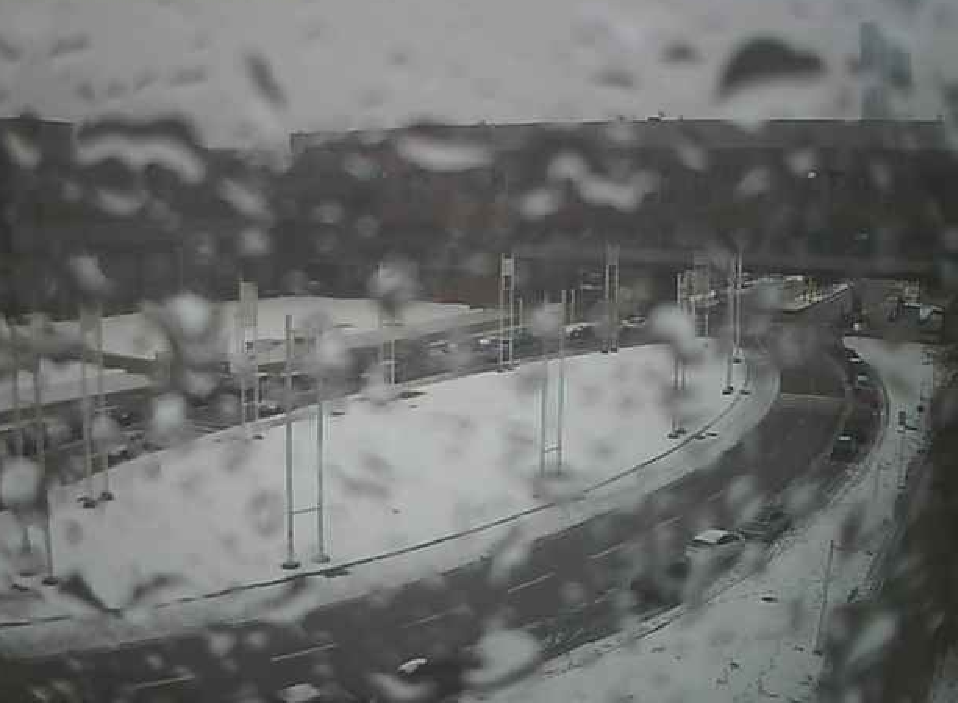
\includegraphics[width=0.225\linewidth]{Immagini/pioggia}}
\subfigure[]{\label{fig:neve} 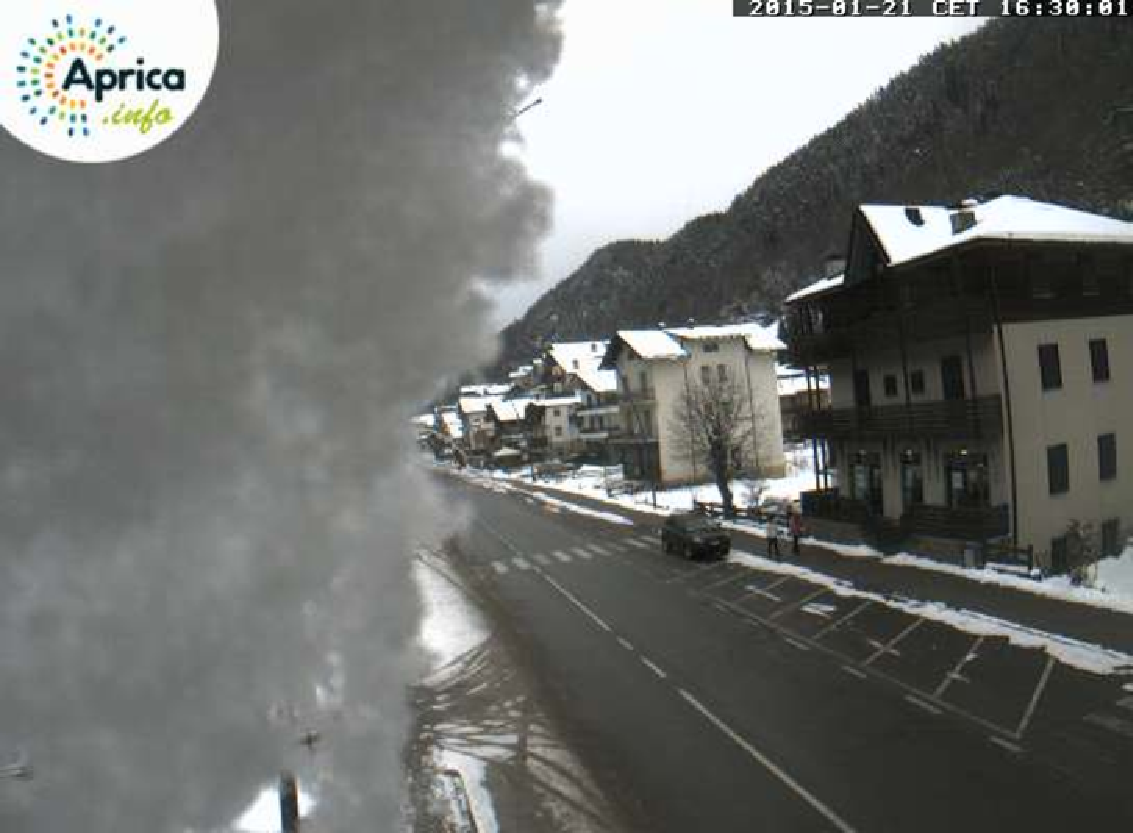
\includegraphics[width=0.225\linewidth]{Immagini/neve}}
\subfigure[]{\label{fig:displ1} 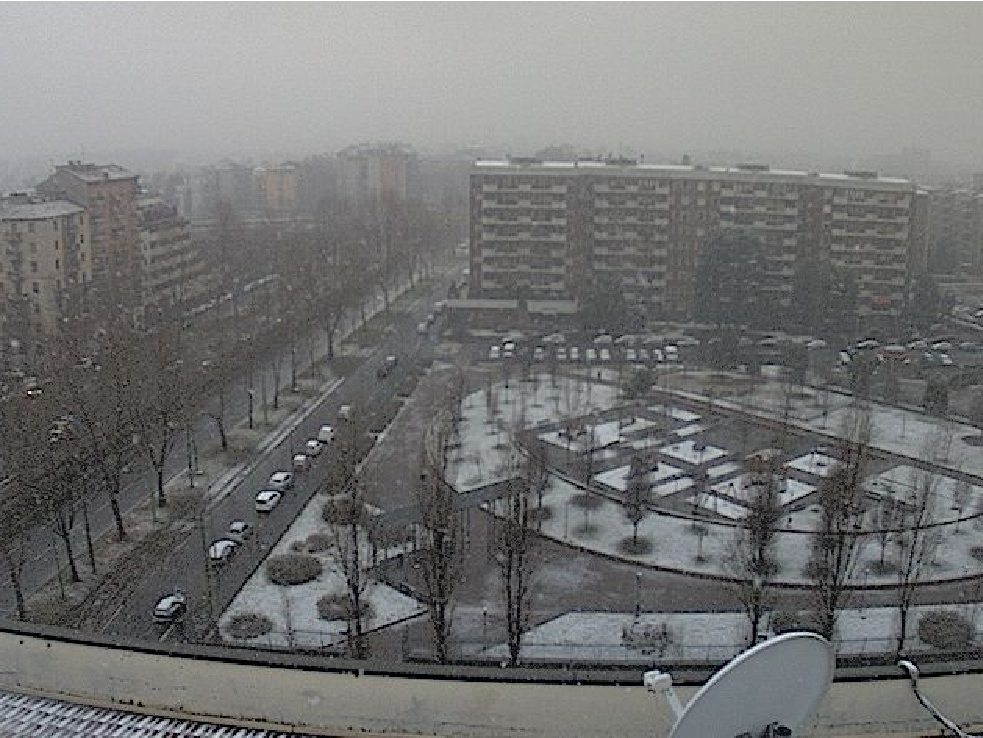
\includegraphics[width=0.225\linewidth]{Immagini/displ1}}
\subfigure[]{\label{fig:displ2} 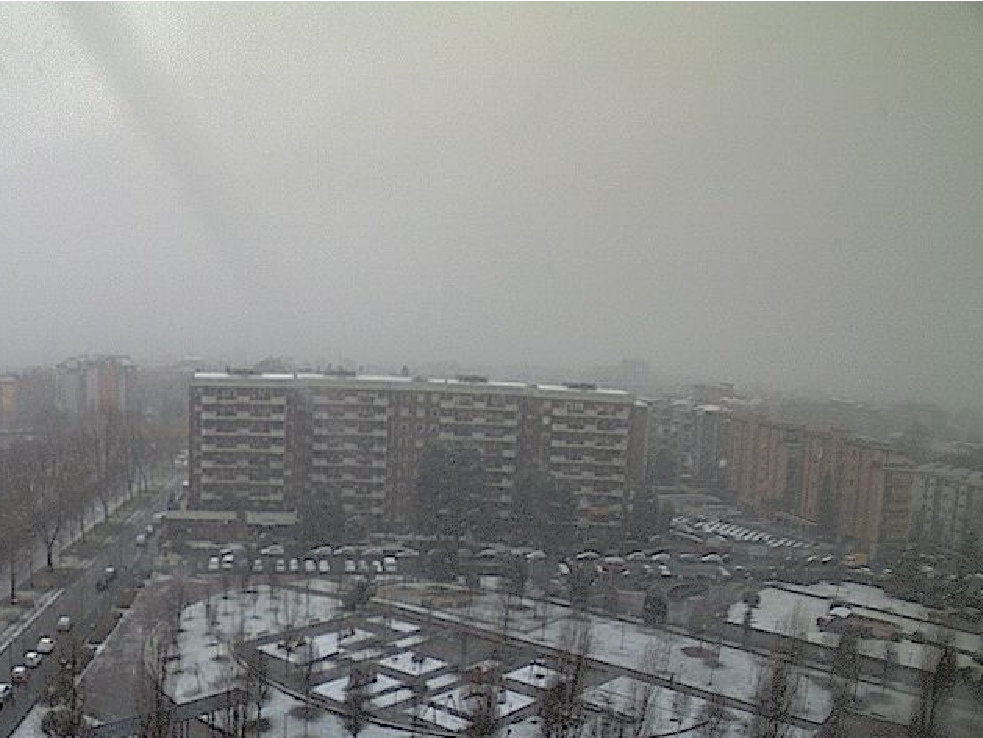
\includegraphics[width=0.225\linewidth]{Immagini/displ2}}
\caption{Examples of tampering events due to atmospheric phenomena. \textbf{(a)} rain drops resulting in a blurry picture, \textbf{(b)} snow partially occluding the camera view, \textbf{(c)}-\textbf{(d)} wind displacing the camera.}
\label{fig:tampering}
\end{figure}

% Why is it interesting and important?
Tampering detection is an essential feature in surveillance systems~\cite{hampapur2005smart}, which are expected to autonomously detect any tampering, and promptly report alerts. Tampering, in fact, might result in images that are useless for monitoring purposes: even a mild blur might hinder the identification of important details such as licence plates. Surveillance cameras most often operate at normal frame-rates (e.g. around few frames per second) and are connected to the power supply. Tampering detection for surveillance cameras have been quite investigated in the literature; in particular, camera displacements and occlusions are typically detected by comparing the current frame against an estimate of the scene background, while blurring is detected by monitoring the high-frequency components of images, as these are expected to drop. In~\cite{aksay2007camera} and~\cite{saglam2009real} tampering is detected by comparing the histograms of background and current frame, and by monitoring the energy in wavelet or Fourier domain. Two background models, estimated over different time intervals, are used in~\cite{saglam2009real}. In~\cite{gil2007automatic}, tampering detection is performed by combining background subtraction together with edge detection and normalized cross-correlation. Background estimates and block matching in~\cite{tsesmelis2013tamper} enable the displacement detection, while the number of SURF~\cite{bay2006surf} keypoints is used to detect blurring. A buffer of recent frames rather than an explicit background can be used as in~\cite{ribnick2006real}. All the above solutions, including~\cite{harasse2004automated,kryjak2012fpga}, are computationally demanding and are not viable options for low-power cameras.

In this work, we expressly target low-power and ultra-low-power smart cameras, like \emph{SecSoC} (Security System on Chip), an innovative prototype based on a cluster of ReISC (Reduced Energy Instruction Set Computer) cores, designed and produced by STMicroelectronics. SecSoC is a battery-powered device, characterized by a constrained computational power (clock rates 82.5 MHz at 1.2V, and sub-1MHz at 0.6V) and reduced memory (1.25 MB). While low-power cameras are not meant for critical surveillance applications, they might be easily employed for monitoring wide environments thanks to their low cost and maintenance requirements.  %As an example, consider Wireless Multimedia Sensor Networks (WMSN) \cite{akyildiz2007survey} where smart-cameras can acquire and transmit images at regular time interval or upon requests. 
% These units are not connected to the power supply and have to operate with batteries and possibly rely on energy harvesting~\cite{magno2009adaptive}. 
%In practice, because of energy constrain, low-power devices have to operate at very low frame-rates: possibly less than one frame every minute.  

% Why is it hard? (E.g., why do naive approaches fail?)
Tampering detection in low-power cameras (eventually organized in wireless sensor network) is more challenging than in conventional surveillance systems, and this problem has not been much investigated so far~\cite{perrig2004security,alippi2010detecting}. Beside computational aspects -- such as the number of operations per pixels allowed -- the big issue is that low-power smart cameras typically operate at very low-frame rates (e.g., less than one frame per minute), thus the acquired sequence does not evolve smoothly. These aspects prevent the use of learned background models and the analysis of foreground variations. In fact, when dynamic environments are monitored at low frame-rates, changes in the scene and in the light conditions might produce consecutive frames that are very different (see Figure~\ref{fig:sequences}). Smart cameras have to promptly distinguish between \emph{normal} changes (due to illumination or movements in the scene), and changes due to camera tampering, to raise an alert and eventually avoid the transmission of tampered frames. %Moreover, false alarms represent a serious problem in low-power smart cameras since they result in energy waste because of useless data processing and unnecessary network transmissions.
% We here address the problem of detecting tampering events on a camera device that is employed for monitoring purpose. Tampering events can be due to malicious attacks, as for instance a displacement of the camera or spraying some dirty liquid that would prevent the acquisition of (part of) the monitored scene or the interpretation of the content (e.g., the identification of licence plates). 

%What are the key components of my approach and results? Also include any specific limitations.
We address the detection of camera blurring and displacement (Section \ref{sec:probForm}), and propose an algorithm (Section~\ref{sec:propSol}) that relies on indicators that can be easily computed in low-power smart cameras. We monitor the average image intensity or frame difference (to detect camera displacement), and the average gradient norm (to detect blurring), and detect tampered frames by analyzing outliers in these indicators. In particular, we show that separately monitoring these indicators over different regions of the image can substantially improve the displacement-detection performance. Image regions are defined during an initial configuration phase (Section \ref{subsec:Segmentation}), thus the algorithm operates at a negligible computational overhead with respect to monitoring the whole image (Section \ref{subsec:coputationalComplexity}). Our algorithm thus represents a prompt trigger, to be possibly combined with other sequential monitoring techniques. Experiments (Section \ref{sec:experiments}) show that leveraging image regions can substantially improve the displacement-detection performance. % Concluding remarks and discussions are given in Section \ref{sec:Conclusion}.


%A low-complexity and sequential monitoring scheme over the average gradient norm is used in~\cite{alippi2010detecting} to detect blurring due to external disturbances on the camera lens.

%\subsection{Related Works}\label{subsec:relWorks}
%% The literature concerning tampering detection is mostly focused on video surveillance applications and process at few frames per second.
% 
%%
%: comparison between frames belonging to a buffer in order to find high values of dissimilarity, associated to tampering.
%\cite{harasse2004automated}: tampering detection inside a moving vehicle; uses background subtraction methods in order to identify defocus, occlusions, and displacements. Comparison of edges pixels count for defocus detection, entropy comparison for occlusion detection, block matching algorithm for displacement detection.
%
%
%
\section{Problem Formulation}\label{sec:probForm}
%
Let $z_t$ be frame acquired at time $t$
\begin{equation}
\label{eq:observationModel}
z_t(x)=\mathcal{D}_t[y_t](x), \quad \forall x \in X
\end{equation}
where $\mathcal{D}_t$ denotes an operator transforming the original image $y_t$, and $x\in \mathbb{Z}^2$ indicates the pixel coordinates belonging to the regular pixel grid $X \subset \mathbb{Z}^2$. As far as there are no tampering attacks/events,
\begin{equation}
\label{eq:no_tampering}
\mathcal{D}_t[y_t](x) = y_t(x) + \eta_t(x), \quad \forall x \in X
\end{equation}
where $\eta_t$ is a random variable accounting for image noise and $y_t$ are acquired from the same viewpoint and camera orientation, even though typically $y_t \neq y_{t-1}$ because the depicted scene changes.\\
When, at time $\tau^*$, an external disturbance introduces \emph{blurring}, the image $y_t$ is degraded by an unknown blur operator, and $z_t$ becomes
\begin{equation}
\label{eq:model_defocus}
\mathcal{D}_t[y_t](x) = \int_{\mathcal{X}}y(s)h_t(x,s)ds\, + \eta_t(x) \quad \forall x \in X, t \geq \tau^*
\end{equation}
where $h_t(x,\cdot) > 0$ is the point-spread function at pixel $x \in X$.\\
A \emph{camera displacement} at frame $\tau^*$ is instead modeled as 
\begin{equation}
\label{eq:model_displacement}
z_t(x)  = \left\{ \begin{array}{rcl}
y_t(x) + \eta(x) & \mbox{per} & t < T^* \\
w_t(x) + \eta(x) & \mbox{per} & t \geqslant T^*
\end{array}\right. ,
\end{equation}
where $w_t$ and $y_t$ refer to different viewpoints and/or camera orientations.

The proposed tampering-detection algorithm analyzes a sequence of frames $\{z_t, t=1,\dots\}$ to detect the time instant $\tau^*$ when tampering like \eqref{eq:model_defocus} or \eqref{eq:model_displacement} occurs. We assume that $T_0$ tampering-free frames are provided for training. For simplicity, we consider grayscale frames: extensions to color images are straightforward.

\begin{figure}[t]
\centering
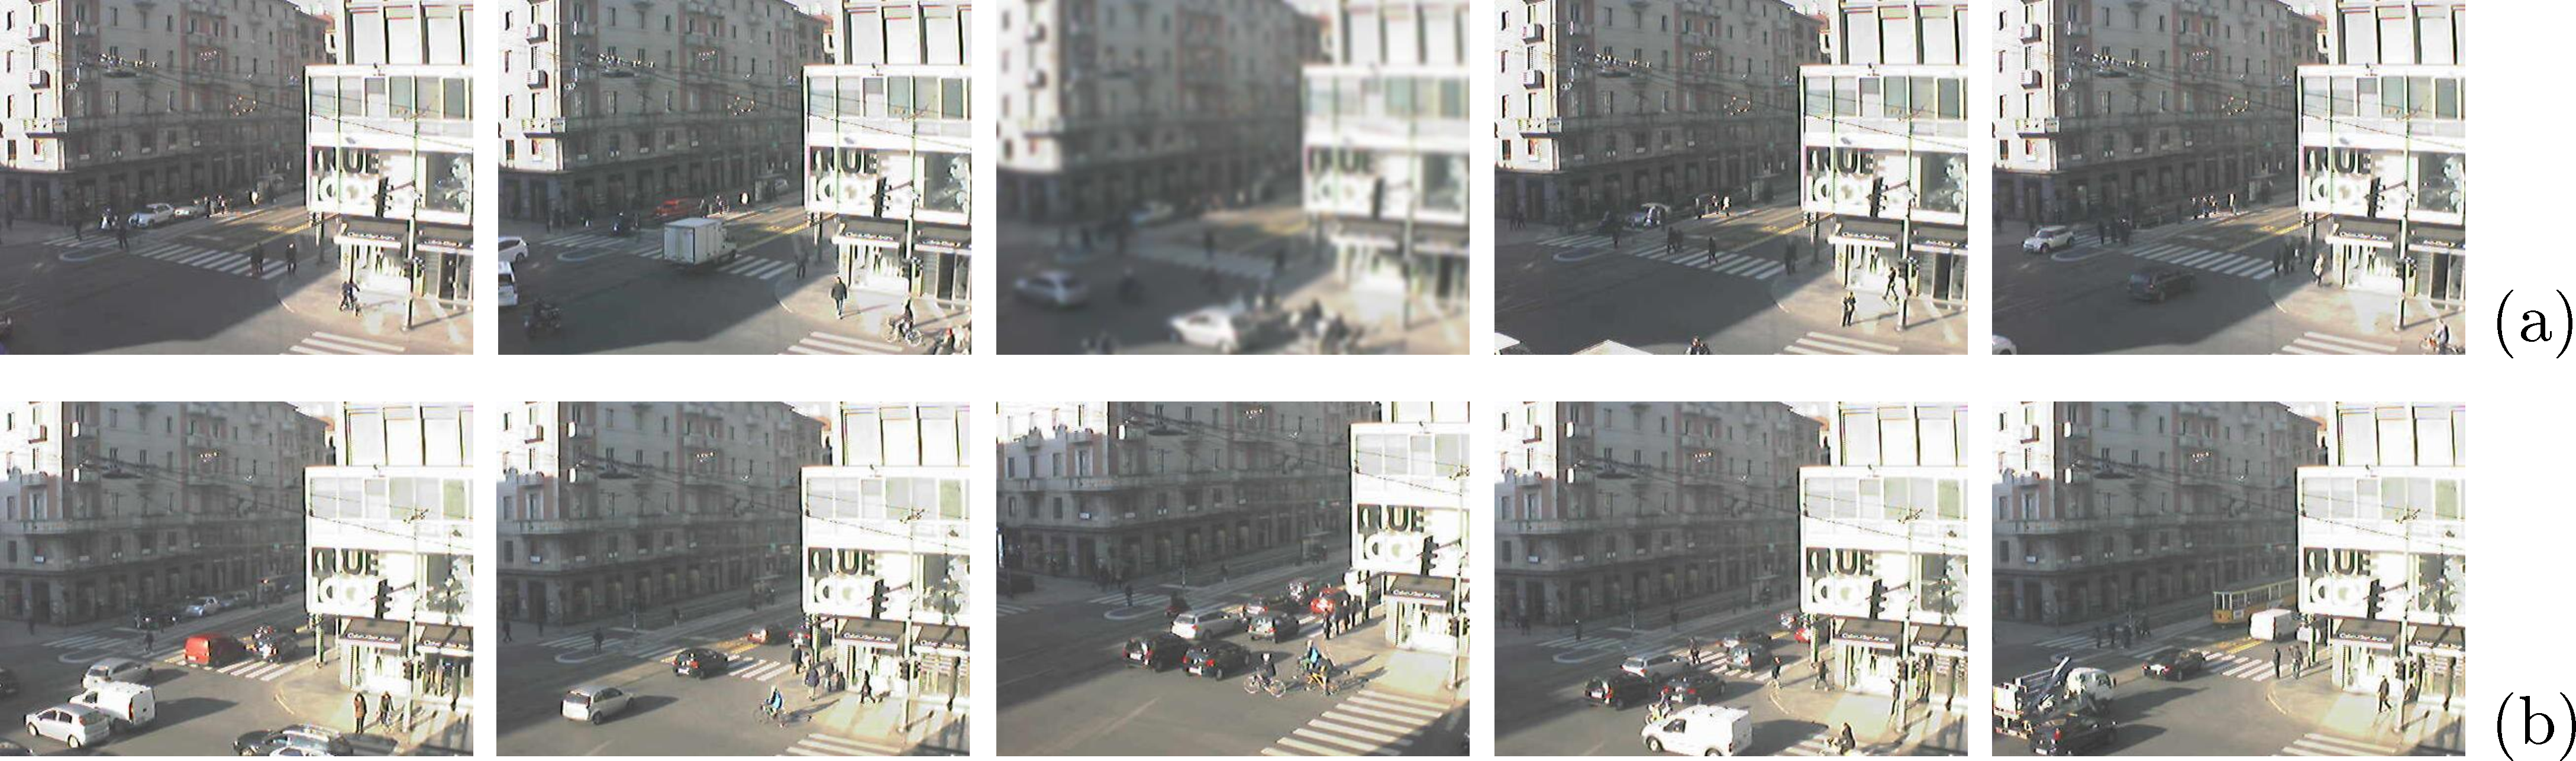
\includegraphics[width=1\linewidth]{Immagini/sequenze}
\caption{Examples of synthetically generated blurring (3-rd frame in \textbf{(a)}) and camera displacement (3-rd frame in \textbf{(b)}).}
\label{fig:sequences}
\end{figure}

\section{Tampering Detection}\label{sec:propSol}

Algorithm~\ref{alg:DISPL} presents the proposed tampering detection, which relies on simple indicators such as the average intensity (the \emph{luma}, denoted by $l$), the average frame difference (denoted by $d$) and the average norm of the gradient (denoted by $g$). The first two are meant to detect camera displacements, which would substantially change the image content, while the latter the blurring, which would cause a drop of the energy in the high-frequencies. As anticipated in Section~\ref{sec:introduction}, during the initial configuration, the scene is segmented in $K$ disjoint regions $\{R_k, k = 1,\dots,K\}$, namely $R_k \subset \mathcal{X}, R_i \cap R_j = \emptyset, \forall i \neq j$. The employed segmentation is detailed in Section~\ref{subsec:Segmentation}. 

For each $z_t$, we compute the luma and frame difference (FD) separately on each of the $K$ regions,
\begin{eqnarray}
\vspace{-0.5cm}
l_k(t) &=& \frac{1}{\#R_k} \sum_{x \in R_k} z_t(x) \label{eq:lumaRegions}\\
d_k(t) &=&\frac{1}{\#R_k} \sum_{x \in R_k} \left(z_t(x) - z_{t-1}(x) \right)^2, \ \ k = 1, \dots, K\,,\label{eq:FDRegions}
\vspace{-0.5cm}
\end{eqnarray}
where $\#(\cdot)$ denotes the cardinality of a set. We can simultaneously monitor both luma and frame difference, even though computing $d_k$ requires to store the previous frame and this also depends on memory availability of the device. In what follows, including Algorithm~\ref{alg:DISPL}, we consider only the luma $l$, but the same procedures apply to the frame difference $d$ as well. The average gradient norm is instead computed over the whole image
\begin{equation}
\label{eq:normaGradiente}
g(t) = \sum_{x \in X} \left (\sqrt{\left(z_t \circledast f_h\right)^2(x) + \left(z_t \circledast f_v\right)^2(x)}\right),
\end{equation}
where $f_h$ and $f_v$ are the horizontal and vertical derivative filters, respectively, and $\circledast$ denotes the 2d convolution. 

\begin{figure}[tb]
\centering
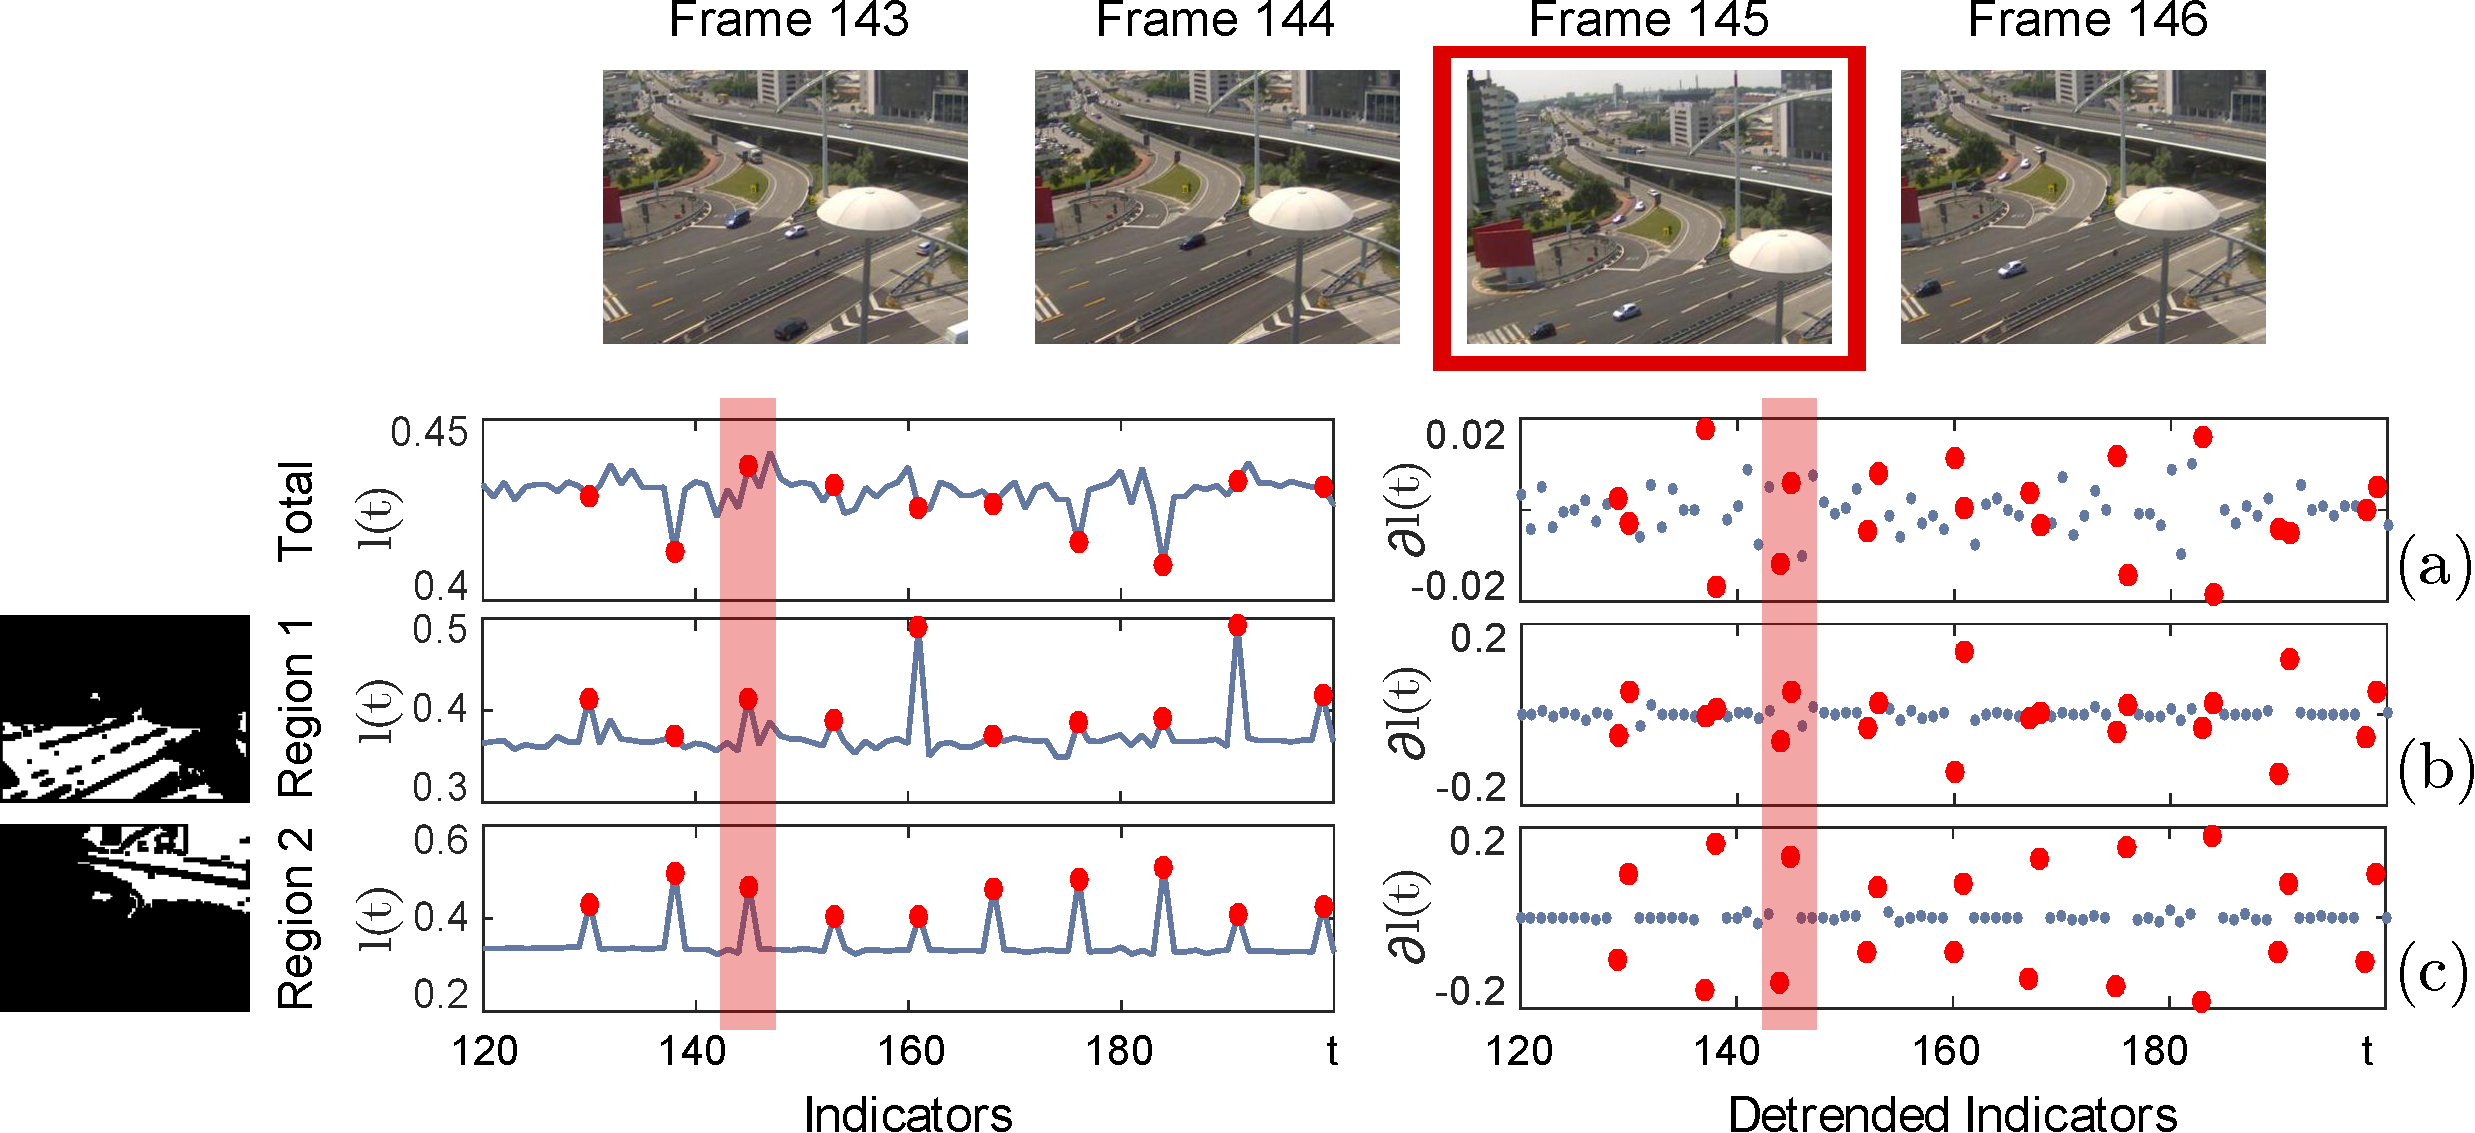
\includegraphics[width=1\linewidth]{Immagini/indicatori}
\caption{Example of camera displacements. 
Left plots report the luma values, while right plots depict the detrended luma: 
we show both indicators computed over the full image (\textbf{a}) and on two reported regions (\textbf{b} and \textbf{c}). Red dots indicate a single displaced frame. Values in the highlighted areas refer to the frames depicted on top of the figure. 
Displacement yields a peak in $l$ and two outliers in the sequence of detrended indicators $\partial l$, which can be clearly detected.}
\label{fig:indicatori} 
\end{figure}
%Tampering changes the sequence of indicators:
Figure~\ref{fig:indicatori} shows how a camera displacement affects the luma. First of all, we observe that a displaced frame changes $l(t)$ (introducing a peak in Figure~\ref{fig:indicatori}(a)) and that this change is also visible in the indicators $l_k(t)$ for the regions (Figure~\ref{fig:indicatori}(b) and Figure~\ref{fig:indicatori}(c)). Second, we observe that outlier-detection methods~\cite{Chandola2009} based on density estimates or on confidence intervals --that are very efficient to run-- cannot be straightforwardly applied here. In fact, these methods are meant for independent and identically distributed (i.i.d.) random variables, while here indicators follow an unpredictable trend because of changes in the scene or in the illumination. Therefore, we perform a detrending~\cite{Gustafsson2000} of the indicator sequence by a temporal derivative
\begin{equation}\label{eq:detrending}
 \partial l_k(t) = l_k(t)-l_k(t-1),  \ \ k = 1, \dots, K\,,
\end{equation}
and we similarly define $\partial d_k(t)$ and $\partial g(t)$. 

\begin{algorithm}[t]
	% \SetAlgoNoLine
	\LinesNumbered
	\SetAlgoNlRelativeSize{0}
	\SetNlSty{small}{}{.}
	\textbf{Input}: $\gamma_l, \gamma_g, \Gamma_l$, training frames $\{z_t, t = 1, \dots, T_{0}\}$, regions $\{R_k, \ k=1,\dots,K\}$ \\
	\textbf{Training phase}:\\
	\lnl{DISPL-Tr1} Compute $\partial l_k(t)$ and $\partial g(t), t = 1, \cdots, T_o$\\ 
	\lnl{DISPL-Tr7} Compute $\overline{\partial l}_k$, $\overline{\partial g}$, $\sigma_{l_k}$ and $\sigma_{g}$.\\
	
	\textbf{Operational phase}:\\
	\lnl{DISPL-Test1} \For{$t=T_{o} + 1,\dots,\infty$}{
		\lnl{DISPL-Test2} Get frame $z_t$, set $n_l =0$;\\
		\lnl{DISPL-Test10} Compute $\partial g(t)$\\
			\lnl{DISPL-Test11} \If{$\partial g(t) < -\gamma_g \sigma_{g} \vee \partial l(t) > \gamma_g \sigma_{g} $}{
					\lnl{DISPL-Test9} raise a blurring alert in $z_t$ \\
									}
		\lnl{DISPL-Test4} \For{$k=1,\dots,K$}{
			\lnl{DISPL-Test5} Compute $\partial l_k(t)$\\
			\lnl{DISPL-Test6} \If{$\partial l_k(t) < -\gamma_l \sigma_{l_k} \vee \partial l_k(t) > \gamma_l \sigma_{l_k} $}{
				\lnl{DISPL-Test7} $n_l=n_l+1$\\
			}
		}
		\lnl{DISPL-Test8} \If{$n_l\geq \Gamma_l$}{
			\lnl{DISPL-Test9} raise a camera displacement alert in $z_t$ \\
		}
	}   
	\caption{The Proposed Tampering-Detection Algorithm}
	\label{alg:DISPL}
\end{algorithm}

The sequences of detrended indicators (reported in Figure~\ref{fig:indicatori}) can be suitably monitored by the following confidence intervals:
\begin{equation}\label{eq:confidenceRegions}
 [\overline{\partial l}_k(t) - \gamma_l \sigma_{l_k}, \overline{\partial l}_k(t) + \gamma_l \sigma_{l_k}], \ \  k = 1,\dots,K\,,
\end{equation}
where $\overline{\partial l}_k(t)$ denotes the mean and $\sigma_{l_k}$ the standard deviation of $\partial l$ over $R_k$ (Algorithm~\ref{alg:DISPL}, line \ref{DISPL-Tr1}), computed from tampering-free frames provided for training (i.e. $z_t\,, t = 1, \dots, T_o$) and $\gamma_l >0$ is a tuning parameter. Similar intervals are built for  $\partial d_k(t)$ and $\partial g$ (line~\ref{DISPL-Tr7}). 

During operations, indicators are computed (lines~\ref{DISPL-Test10} and~\ref{DISPL-Test5}), and any indicator falling outside its confidence region is considered an outlier. In particular, any outlier in $\partial g$ yields a blurring alert (line~\ref{DISPL-Test11}), while camera-displacement alerts are raised when at least $\Gamma_l$ indicators $\partial l_k$  simultaneously yield outliers (line~\ref{DISPL-Test8}). The threshold $\Gamma_l$ together with $\gamma_l$ determine the displacement-detection promptness. The extreme configurations correspond to $\Gamma_l = 1$, where it is sufficient that a single region fires an outlier to raise a camera-displacement alert, and $\Gamma_l = K-1$ where all but one region\footnote{It is better to exclude a region since, for instance, the sky-region typically does not change when the camera is displaced, either horizontally or vertically} have to simultaneously fire an outlier to raise an alert.

It is important to remark that tampering yields outliers in the transient of the detrended indicators~\eqref{eq:detrending}: namely, a single tampered frame yields two outliers (as shown in Figure~\ref{fig:indicatori}) and only the first and the last of a sequence of consecutive tampered frames yield outliers in the detrended indicators. This is the reason why detrended indicators are monitored in a one-shot manner, targeting the detection of the first tampered-frame. On the one hand, this one-shot solution can provide prompt detections, which is particularly important at the low frame-rates we consider, on the other hand, the persistence of tampering is disregarded. To take this valuable information into account, some form of sequential monitoring should be applied to the indicator sequence as in~\cite{alippi2010detecting}, possibly combined with the proposed one-shot monitoring.
%
%
\subsection{Scene Segmentation}\label{subsec:Segmentation}
Scene has to be preliminarily segmented to define regions that Algorithm \ref{alg:DISPL} takes as input. To this purpose, we use part of the training frames before $T_0$ to compute the feature vector $\textbf{f}(x)\in \mathbb{R}^5$ for each pixel $x\in\mathcal{X}$ 
\begin{equation}
\label{eq:featureVector}
\textbf{f}(x)=\left[r(x);c(x);\bar{l}(x);\sigma_{l}(x);\overline{g}(x);\sigma_{g}(x)\right]\,, \ \forall x \in X\,.
\end{equation}
In \eqref{eq:featureVector}, $r(x)$ and $c(x)$ denotes the row and column of $x$, respectively, $\bar{l}(x)$ and $\sigma_{l}(x)$ the mean and standard deviation of the intensity at $x$, computed over time, and $\overline{g}(x)$ and $\sigma_g(x)$ the mean of gradient norm and its standard deviation, computed over time. These feature vectors are meant to cluster pixels in regions having, over training frames, similar spatial appearance and temporal behavior.

As in superpixel methods \cite{Susstrunk2012}, segmentation is performed by k-means clustering. Feature vectors~\eqref{eq:featureVector} over the whole image are clustered by a weighted k-means~\cite{kottke1994motion} that scales each component of the Euclidean distance between a feature vector and a cluster centroid of a weight that is inversely proportional to the standard deviation over the cluster. This scaling compensates the fact that feature vector components might span very different ranges. The number of clusters is defined by testing several values and then choosing the best solution according to the Calinski-Harabasz criterion~\cite{calinski1974dendrite}.

%\gi{Adriano, controlla bene}
%The number of clusters is defined by the Calinski-Harabasz criterion~\cite{calinski1974dendrite}, which initializes the weighted k-means using different number of clusters, and then chooses the best one according a cost function\gi{Adriano controllare come lo chiama}. 


Finally, morphological image-processing operations are executed to remove boundaries between different regions, and eventually regions that are too small. This defines the regions $\{R_k\,, \ k=1,\dots,K\}$, and two examples are reported in Figure~\ref{fig:indicatori}.

\subsection{Computational Complexity}\label{subsec:coputationalComplexity}

The most computationally demanding operations of Algorithm \ref{alg:DISPL} consist in computing the indicators, in particular $g$. Computing $g$ requires, when using the Sobel filters in~\eqref{eq:normaGradiente}, $34$ operations per pixels\footnote{Execution can be accelerated whether hardware implementations of the FFT transform are available}, while computing $l$ and $d$ requires 1 and 3 operations per pixel, respectively. Detecting outliers in the indicators requires two comparisons per frame: thus, monitoring regions instead of the whole image has a negligible impact on the overall computational complexity. Algorithm~\ref{alg:DISPL} has very low memory requirements: $l$ and $g$ indicators can be computed online, while $d$ requires to store a single frame in memory. Segmentation is executed only during the initial configuration and can be performed on an external device connected to the smart camera. As such, Algorithm~\ref{alg:DISPL} can be properly executed on low-power and ultra low-power cameras.
%\gi{Adriano: inserisci qui l'algoritmo e traducilo in inglese. Se riusciamo lo spostiamo prima di tutte le sottosezioni}
\vspace{-0.2cm}
\section{Experiments}\label{sec:experiments}
Experiments are meant to assess the advantages of separately monitoring regions in the considered tampering-detection framework. To this purpose, we show that Algorithm~\ref{alg:DISPL} detects camera displacements better than monitoring indicators on the whole image (\emph{Whole Image} in Figure~\ref{fig:ROC}). We also show that it is important to define regions considering the scene content, since operating on $K$ regions obtained by clustering $[r(x), c(x)]$ leads to performance loss (\emph{Voronoi} in Figure~\ref{fig:ROC}). For both Voronoi and regions defined as in Section~\ref{subsec:Segmentation}, we consider the two extreme configurations where alerts are raised at the first region firing an outlier or when $K-1$ regions simultaneously fire outliers.

We recorded $8$ sequences from webcams monitoring different urban areas, yielding overall $12200$ frames. From each frame we have cropped the central area, removing the 50 top-most and bottom-most rows, and the 50 left-most and right-most columns\footnote{Sequences can be provided upon request.}. We have synthetically introduced $10\%$ of tampered frames: displacements have been simulated by moving the central cropping area of a random shift having magnitude between 20 and 50 rows and coulumns (as in Figure \ref{fig:sequences}(b)). Blurring  (as in Figure \ref{fig:sequences}(a)) was simulated by convolution against a Gaussian kernel, with $1\leq\sigma\leq5$ randomly defined. 
%\gi{Adriano: image sizes? blur kernel std? quanti pixel il displacement?}
%The second dataset was recorded using a Raspberry Pi Model B+ \cite{raspberry} mounting a camera module. 
%Few sequences of the first dataset contain real tampering events  (Figure \ref{fig:indicatori}). 
%In the second dataset, tampering was introduced by moving the device or spraying water on the camera lens. 

A typical figure of merit for assessing detection performance is the Receiver Operating Characteristic (ROC) curve, where each point corresponds to a pair (FPR$_\gamma$, TPR$_\gamma$) defined as
%
\[\text{FPR}_\gamma = \frac{\text{FP}_\gamma}{\text{TN}_\gamma+\text{FP}_\gamma}, \ \text{ and } \ \text{TPR}_\gamma=\frac{\text{TP}_\gamma}{\text{TP}_\gamma+\text{FN}_\gamma}.\]
%
Here, TP$_\gamma$ represents the number of true positives (tampered frames correctly detected), FP$_\gamma$ of false positives (tampering-free frames detected), TN$_\gamma$ of true negatives (tampering-free frames not detected) and FN$_\gamma$ of false negatives (missed tampered frames), for a given value of $\gamma$. ROC curves have been computed by varying $\gamma_l$, $\gamma_d$ and $\gamma_g$ in a range of values between $0.1$ and $50$. 
\vspace{-0.3cm}
\subsubsection{Discussion}
ROC curves in Figure~\ref{fig:ROC}(a)-(b) and the Area Under the Curve (AUC) values reported in the caption confirm that camera displacements can be better detected by monitoring FD than luma, and that it is convenient to define regions segmenting the scene content. As an example, if we set $\gamma_d = 15.6$, Algorithm~\ref{alg:DISPL} operates at $\text{FPR} = 1\%$ and detects nearly all tampering since $\text{TPR} = 99.92\%$. In contrast, to achieve $\text{FPR} = 1\%$ when monitoring the whole image, FPR drops to $91.67\%$ ($\gamma_d = 6.5$), and when considering Voronoi to $\text{TPR} = 89.05\%$ ($\gamma_d = 18.64$). When monitoring $l$, Algorithm~\ref{alg:DISPL} achieves TPR~=~$73.98\%$ at $\text{FPR}=1\%$  ($\gamma_d=5.8$), while monitoring the whole image is quite ineffective ($\text{TPR} = 17.85\%$, $\gamma_d=3.7$), and similarly perform Voronoi's regions ($\text{FPR} = 53.02\%$, $\gamma_d=6$). We remark that, in the considered low-power scenario, it is important to operate at low FPR, given the large number of frames that smart cameras have to process over time and the cost of data-transmission in terms of battery power. As far as the values of $\Gamma_d$ and $\Gamma_l$ are concerned, the most effective configuration consists in raising an alert as soon as a single region fires a very clear outlier, which implies setting quite wide intervals~\eqref{eq:confidenceRegions}. This option is also preferable because it enables the detection of partial occlusions of the scene.

%\gi{Aggiornare con i nuovi dati}
%\emph{Considering $d$ as indicator, we observe that to achieve a recall of $98\%$, Algorithm~\ref{alg:DISPL} operates at $0.4\%$ of false alarms, with $\gamma = 24.7$, which is less than one fifth of the whole image solution ($2.2\%$ with $\gamma = 4.6$) and the Voronoi solution ($2.3\%$ with $\gamma = 12.9$).
%On the other side, considering $l$ as indicator, we observe that to achieve a recall of $98\%$, Algorithm~\ref{alg:DISPL} operates at $13\%$ of false alarms, with $\gamma = 2.5$, which is about one sixth of the whole image solution ($75\%$ with $\gamma = 0.1$) and about three fifty than the Voronoi solution ($22\%$ with $\gamma = 1.7 $).
%Having few false alarms is important in a low-power context, considering the high number of frames that have to be processed. Most importantly, false alerts are halved basically at no computational overhead.} \gi{Aggiornare con i nuovi dati}
Figure~\ref{fig:ROC}(c) confirms that blurring is more effectively detected by monitoring the whole image at once. This is probably due to the fact that, typically, regions do not include the most prominent edge of the scene, which are indeed the most informative parts to detect blurring. This is the reason why, in Algorithm~\ref{alg:DISPL}, $g$ is monitored on the whole image.%\gi{aggiungere commento su K-1 vornoi che va meglio?}
x
\begin{figure}[t]
\centering
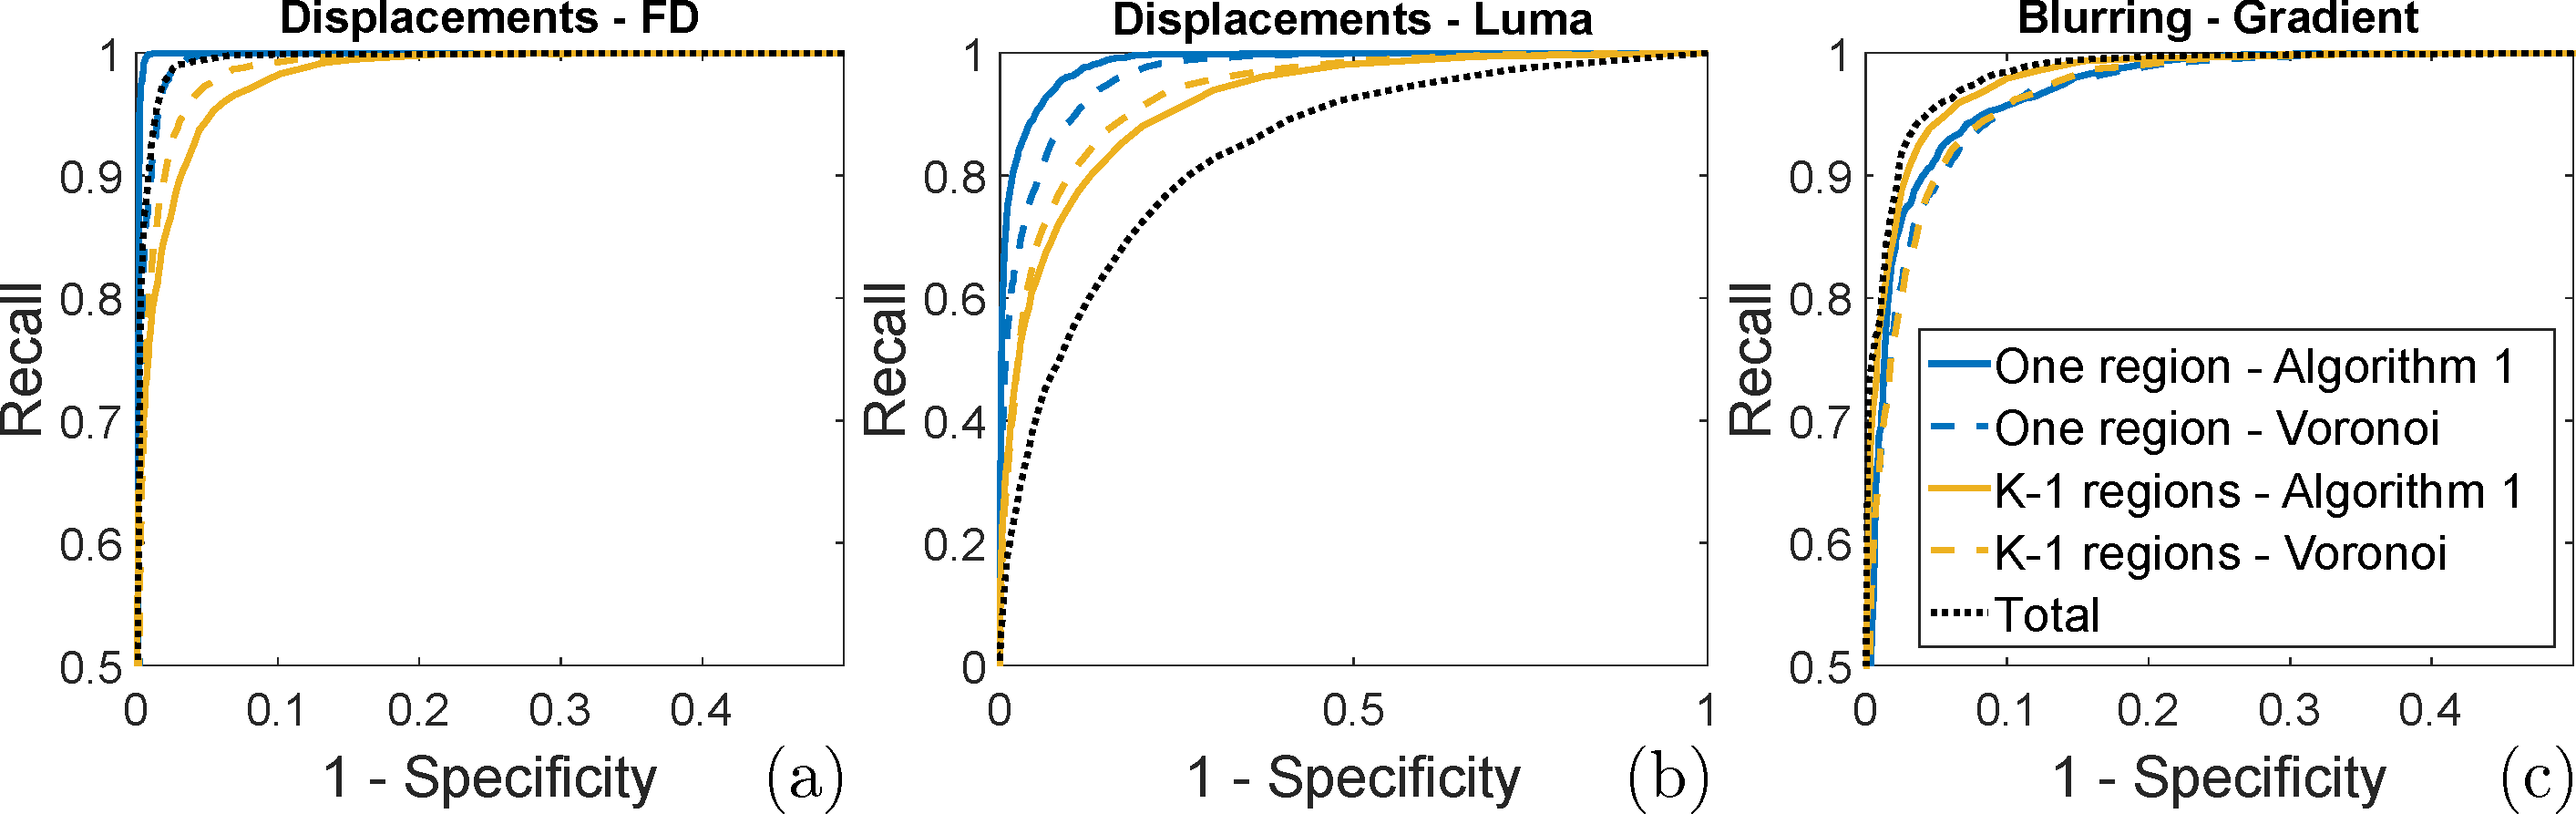
\includegraphics[width=1\linewidth]{Immagini/curve}
\caption{\textbf{(a)} ROC curves relative to displacement detection based on FD: the AUC obtained by 
``Algorithm 1 - One region'' is $99.89\%$, while the AUC obtained by on the whole 
image is $99.65\%$.
\textbf{(b)} ROC curves relative to displacement detection based on luma: the AUC obtained by 
``Algorithm 1 - One region'' is $98.44\%$, while the AUC obtained on the whole 
image is $84.07\%$.
\textbf{(c)} ROC curves relative to blurring detection based on gradient: as opposed to \textbf{(a)} and 
\textbf{(b)}, ``Algorithm 1 - One region'' (AUC $98.4\%$) is outperformed by monitoring the whole image, AUC = $99.13\%$.
To highlight differences, the ROC curves in \textbf{(a)} and \textbf{(c)} are drawn over a smaller FPR, TPR range.}
%\caption{\textbf{(a)} ROC curve for displacement detection considering Frame Difference (FD) as indicator.
%	%There is an improvement in the performance considering adaptive regions w.r.t. considering the whole image or Voronoi regions.
%	The AUC corresponding to Algorithm~\ref{alg:DISPL} ($1$ region - Algorithm $1$) is $99.89\%$, while the AUC of considering the whole image (Total) is $99.65\%$. 
%	%the AUC of Luma-Voronoi is $99.85\%$, and the AUC of Frame-Difference is $99.44\%$ (axis have been zoomed for the visualization sake). Large AUC values indicate that these displacements can be successfully detected and that Algorithm~\ref{alg:DISPL} is the most effective one.
%	\textbf{(b)} ROC curve for displacement detection considering Luma as indicator.
%	%There is an improvement in the performance considering adaptive regions w.r.t. considering the whole image or Voronoi regions.
%	The AUC corresponding to Algorithm~\ref{alg:DISPL} ($1$ region - Algorithm $1$) is $98.44\%$, while the AUC of considering the whole image (Total) is $84.07\%$. 
%	\textbf{(c)} ROC curve for blurring detection.
%	In this case, the Gradient-Total (AUC $99.13\%$) outperforms the Gradient-Regions (AUC $98.4\%$) because this latter do not include the most prominent edges in images, which are the most important information to detect blurring. %This is the reason why, in Algorithm~\ref{alg:DISPL}, $g$ is monitored on the whole image. 
%	ROC curves \textbf{(a)} and \textbf{(c)}
%	%For the visualization sake, ROC curves \textbf{(a)} and \textbf{(c)} have been reported in a limited range of both axis, and in particular we focus on low values of 1-SPECIFICITY, thus of false alarms.
	%}
\label{fig:ROC}
\end{figure}
%\begin{figure}[htb]
%\centering
%\subfigure[]{\label{fig:buenosAiresDef}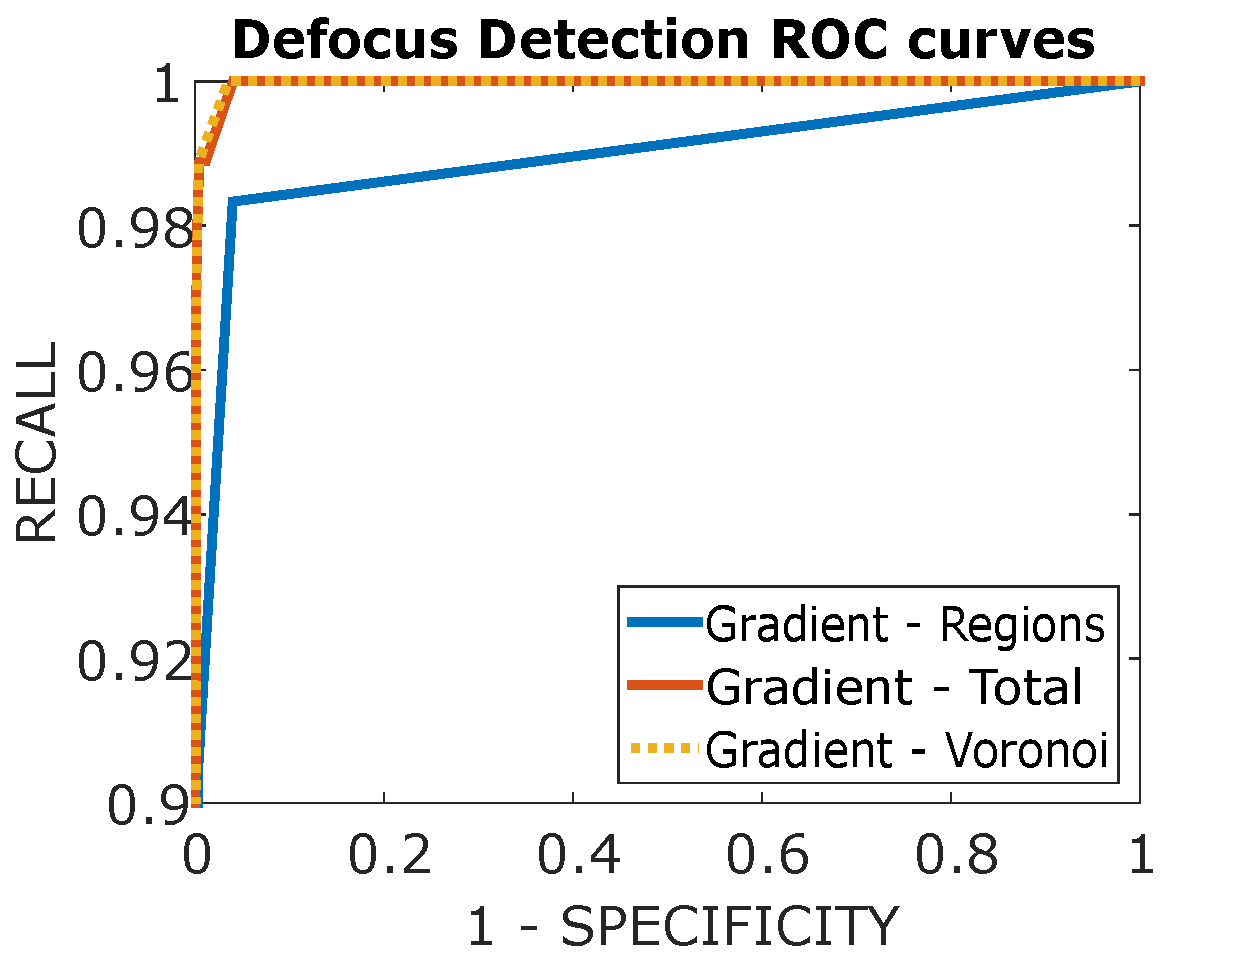
\includegraphics[width=0.45\linewidth]{Immagini/ROCdefocus1}}
%\subfigure[]{\label{fig:buenosAiresDispl} 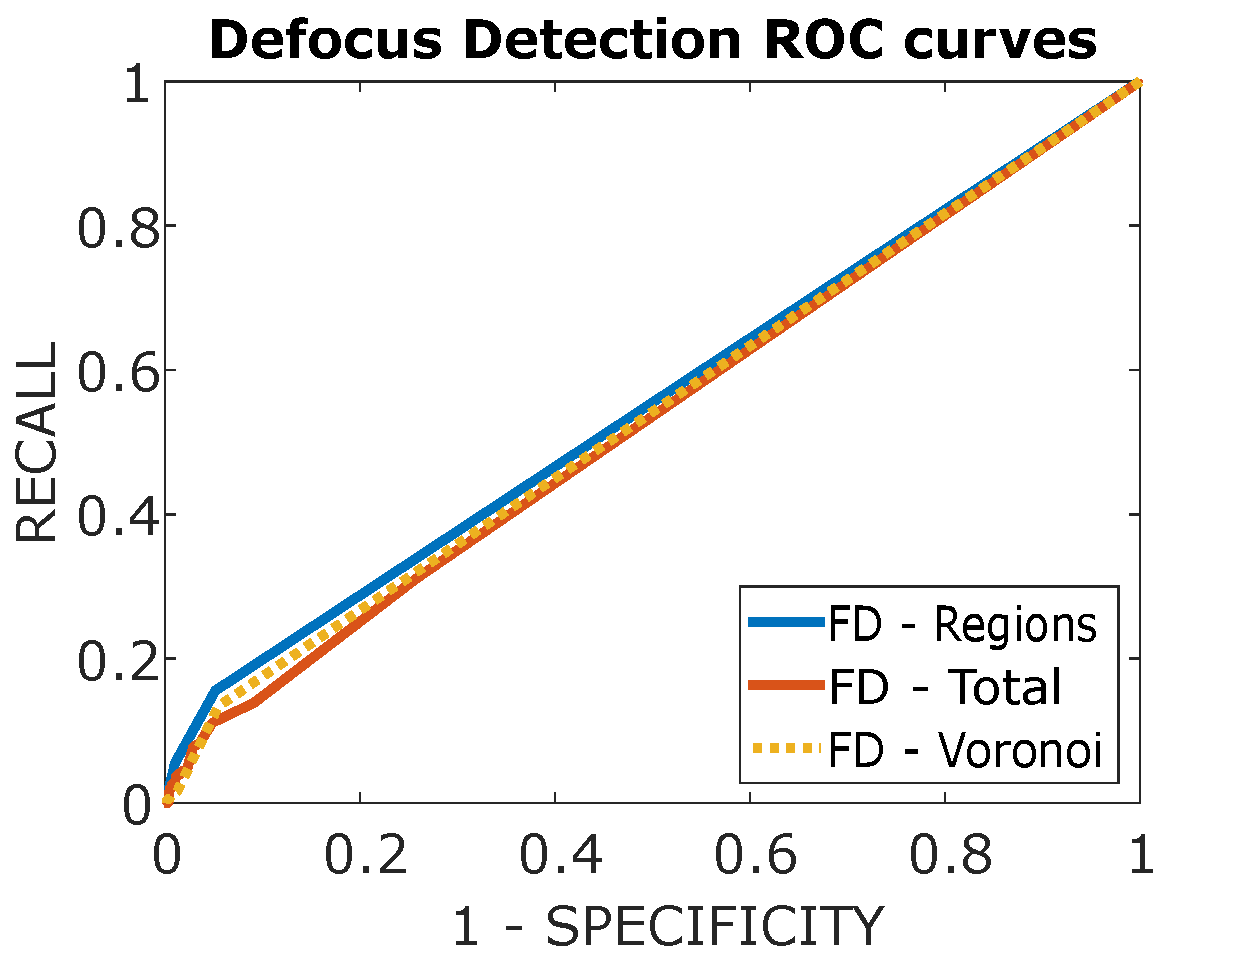
\includegraphics[width=0.45\linewidth]{Immagini/ROCdefocus_fd}}
%\caption{ROC curves for defocus detection, considering three alternative approaches. \textbf{(a)} Analysis of the mean gradient energy. \textbf{(b)} Analysis of the frame differencing.}
%\label{fig:ROCdisplacement}
%\label{fig:ROCdefocus}
%\end{figure}

%
%\begin{table}[tbh]
%\centering
%\begin{tabular}{l|l|l|l|l|l|l|}
%\cline{2-7}
%& \multicolumn{3}{l|}{\cellcolor[HTML]{C0C0C0}\textbf{Displacement Detection}}  & \multicolumn{3}{l|}{\cellcolor[HTML]{C0C0C0}\textbf{Blurring Detection}} \\ \cline{2-7} 
%& \cellcolor[HTML]{EFEFEF}\textbf{Regions} & \cellcolor[HTML]{EFEFEF}\textbf{Total} & \cellcolor[HTML]{EFEFEF}\textbf{Voronoi} & \cellcolor[HTML]{EFEFEF}\textbf{Regions} & \cellcolor[HTML]{EFEFEF}\textbf{Total} & \cellcolor[HTML]{EFEFEF}\textbf{Voronoi} \\ \hline
%\multicolumn{1}{|l|}{\cellcolor[HTML]{EFEFEF}\textbf{Luma}}     & 0.9994 & 0.9989 & 0.9985  &            &            &             \\ \hline
%\multicolumn{1}{|l|}{\cellcolor[HTML]{EFEFEF}\textbf{Gradient}} &  		 &  		  &             & 0.9895 & 0.9996 & 0.9996  \\ \hline
%\multicolumn{1}{|l|}{\cellcolor[HTML]{EFEFEF}\textbf{FD}}         & 0.9974 & 0.9944 & 0.9974  & 0.5526 & 0.5322 & 0.5391  \\ \hline
%\end{tabular}
%\caption{Area under curve of the analized solutions}
%\label{tab:AUC}
%\end{table}

%Numero di operazioni richieste:
%Calcolo di g(t):
%\begin{itemize}
%\item Norma gradiente: 34 FLOP per pixel
%\item Media delle norme del gradiente
%\end{itemize}
%Calcolo di l(t):
%\begin{itemize}
%\item Media dei valori di grigio
%\item Detrending: 1 FLOP per frame
%\end{itemize}
%Monitoraggio one-shot: 2 confronti
%Monitoraggio sequenziale: 
%Ogni 20 frame
%Calcolo intervalli di confidenza: ~70 FLOP
%Confronto tra intervalli di confidenza: 2 confronti
\vspace{-0.3cm}
\section{Conclusions}\label{sec:Conclusion}
\vspace{-0.1cm}
We presented a tampering-detection algorithm that leverages an image segmentation to improve the detection of camera displacements, and that at the same time can detect blurring. The algorithm has low-computational complexity and has to be considered a prompt trigger for detecting tampering in low-power and ultra low-power cameras operating at low frame rates.

Ongoing work concerns approaching other types of tampering, such as degradations of the imaging sensor, and the integration of sequential monitoring schemes~\cite{alippi2010detecting} to detect subtle tampering that persists over time. Moreover, we will investigate the use of superpixels methods~\cite{Susstrunk2012} to perform the preliminary scene segmentation, by including suitable temporal information to the feature vectors.

%Ongoing work regards the.
%Furthermore, we are investigating strategies to improve the detection performance and reduce the number of \textit{FP}s by combination of our solution with other techniques:
%for example we could use sequential techniques on the features, or integrate the frame analysis with the data extracted from MEMS inertial sensors.   


%Random Toughs:
%\begin{itemize}
%\item Better segmentation
%\item tests on larger datasets
%\item The problem of false alarms, radio module activation
%\item Other tampering attacks like obfuscation (??) which might be due to environmental phenomena such as rain, fog and mist over the camera lenses have to be detected by image analysis methods
%\item Displacement can be perceived by MEMS as well but these device alone are prone to false alarms. Visual inspection is necessary to reduce false alarms
%\end{itemize}

%\section*{Acknowledgments}\label{sec:Acknowledgments}
%Authors would like to thank ST for supporting Adriano Gaibotti.

\bibliographystyle{unsrt}
\bibliography{bibl_tesi}

%\begin{thebibliography}{1}
%	
%	\bibitem{Einstein}
%	A. Einstein, On the movement of small particles suspended in stationary liquids required by the molecular-kinetic theory of heat, Annalen der Physik 17, pp. 549-560, 1905.
%	
%\end{thebibliography}
\end{document}



%
%
%
%\subsection{Indicators}\label{subsec:Indicators}

%\begin{equation}
%\label{eq:gradientRegions}
%\begin{array}{ccc}
%g^k(t)&  = & \mathcal{G}^k[z_t] = \frac{\sum_{R_k}\| \nabla z_t(x) \| _2^2 }{|{R_k}|}\\
%\partial g^k(t) & =& g^k(t)-g^k(t-1) 
%\end{array},
%\end{equation}
%
%In particolare, per il calcolo delle derivate orizzontali  abbiamo utilizzato il seguente filtro $f_h$:
%\[f_h = f \circledast \left[ \begin{array}{rcl}
%1 & 0 & -1
%\end{array}\right], \] 
%mentre per il calcolo delle derivate verticali abbiamo utilizzato il seguente filtro $f_v$:
%\[f_v = f \circledast \left[ \begin{array}{r}
%1 \\ 0 \\ -1
%\end{array}\right], \]
%dove abbiamo indicato con $\circledast$ l'operatore di convoluzione.
%Il filtro $f$, invece, \`e ottenuto tramite un campionamento della \textit{funzione gaussiana} $h$, con media $0$ e deviazione standard $\sigma$
%\begin{equation}
%\label{eq:gaussian}
%h(i,j)=\frac{1}{2\pi\sigma^2}\exp\left(-\frac{i^2+j^2}{2\sigma^2}\right),
%\end{equation}
%e ponendo il valore massimo di questa funzione nel centro del filtro.
%Con questi filtri \`e possibile calcolare la \textit{norma del gradiente} nel seguente modo:
%
%Una volta calcolata la norma del gradiente \`e possibile farne la media come specificato in \eqref{eq:energyGradient}.
%Il risultato finale \`e un indicatore \textit{scalare} per ciascun frame acquisito, che pu\`o essere monitorato per individuare eventi di sfocature. 
%In particolare ci aspettiamo che l'evento di sfocatura provochi un abbattimento del valore di $g$.